\documentclass[aspectratio=169,11pt]{beamer}

\usetheme{GFRI}
\usepackage[croatian]{babel}
\usepackage{booktabs}
\graphicspath{{slike/}{logo/}}

% Putanje do logotipa. GF logo ostaje obvezan.
\GFRIsetmainlogo{logo/gflogo.pdf}
\GFRIsetpartnerlogoA{logo/logoipsum-434.png}
\GFRIsetpartnerlogoB{logo/logoipsum-434.png}

% Svaki dodatni logo uključuje se ili isključuje zasebno.
% Zamijenite false s true kada se pripadajući logo koristi.
\GFRIpartnerAtrue
\GFRIpartnerBfalse

\title{Naslov prezentacije}
\subtitle{Podnaslov ili naziv kolegija}
\author{Ime i prezime}
\institute{Sveučilište u Rijeci, Građevinski fakultet}
\date{Rijeka, \the\year.}

\begin{document}

\begin{frame}[plain,t]
  \titlepage
\end{frame}

\begin{frame}{Sadržaj}
  \tableofcontents
\end{frame}

\section{Uvod}

\begin{frame}[plain,t]
  \sectionpage
\end{frame}

\begin{frame}{Svrha predloška}
  \begin{columns}[T,onlytextwidth]
    \begin{column}{0.58\textwidth}
      \begin{itemize}
        \item GF logo prikazuje se na svakom slajdu.
        \item Dva dodatna logotipa imaju zasebne prekidače.
        \item Raspored ostavlja dovoljno prostora za sadržaj.
      \end{itemize}
    \end{column}
    \begin{column}{0.36\textwidth}
      \begin{block}{Napomena}
        Za završnu verziju zamijenite privremene logotipe stvarnim datotekama.
      \end{block}
    \end{column}
  \end{columns}
\end{frame}

\section{Rezultati}

\begin{frame}{Primjer isticanja rezultata}
  \begin{alertblock}{Glavni nalaz}
    Ovdje kratko navedite najvažniji rezultat prikazan na slajdu.
  \end{alertblock}

  \vspace{0.18cm}
  Dodatno objašnjenje treba biti sažeto i izravno povezano s prikazanim nalazom.
\end{frame}

\begin{frame}{Primjer slike}
  \begin{figure}
    \centering
    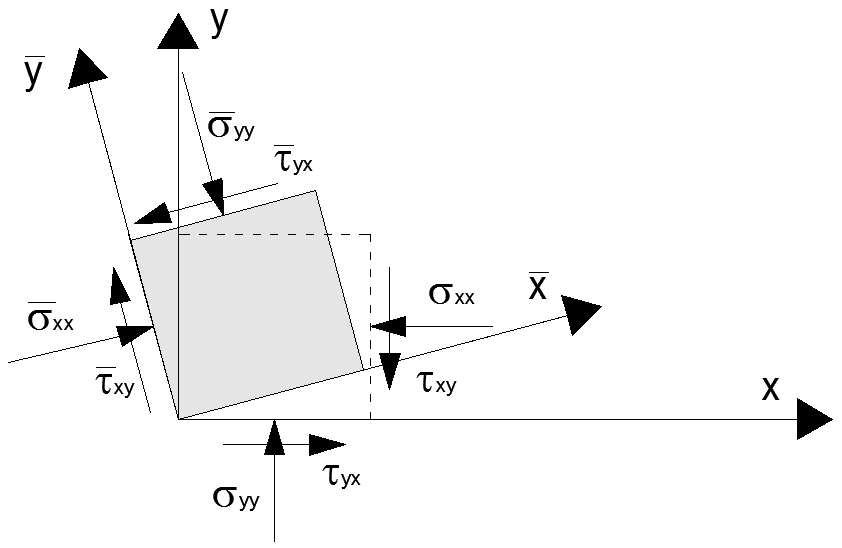
\includegraphics[height=0.57\textheight]{primjer-slike.jpg}
    \caption{Primjer slike učitane iz mape \texttt{slike}.}
  \end{figure}
\end{frame}

\begin{frame}{Primjer tablice}
  \centering
  \begin{tabular}{lrr}
    \toprule
    Pokazatelj & Varijanta A & Varijanta B \\
    \midrule
    Vrijednost 1 & 24,3 & 27,8 \\
    Vrijednost 2 & 18,6 & 17,9 \\
    Vrijednost 3 & 31,2 & 34,1 \\
    \bottomrule
  \end{tabular}

  \vspace{0.40cm}
  {\small\color{GFRISlate}Izvor: navedite izvor podataka ili vlastiti izračun.}
\end{frame}

\section{Zaključak}

\begin{frame}{Zaključak}
  \begin{enumerate}
    \item Sažmite odgovor na glavno pitanje prezentacije.
    \item Navedite ograničenje koje utječe na tumačenje.
    \item Istaknite sljedeći korak ili preporuku.
  \end{enumerate}
\end{frame}

\section*{Hvala na pozornosti}

\begin{frame}[plain,t]
  \sectionpage
\end{frame}

\end{document}
